\subsection{Girlfriend vs Consumer}

\begin{figure}
	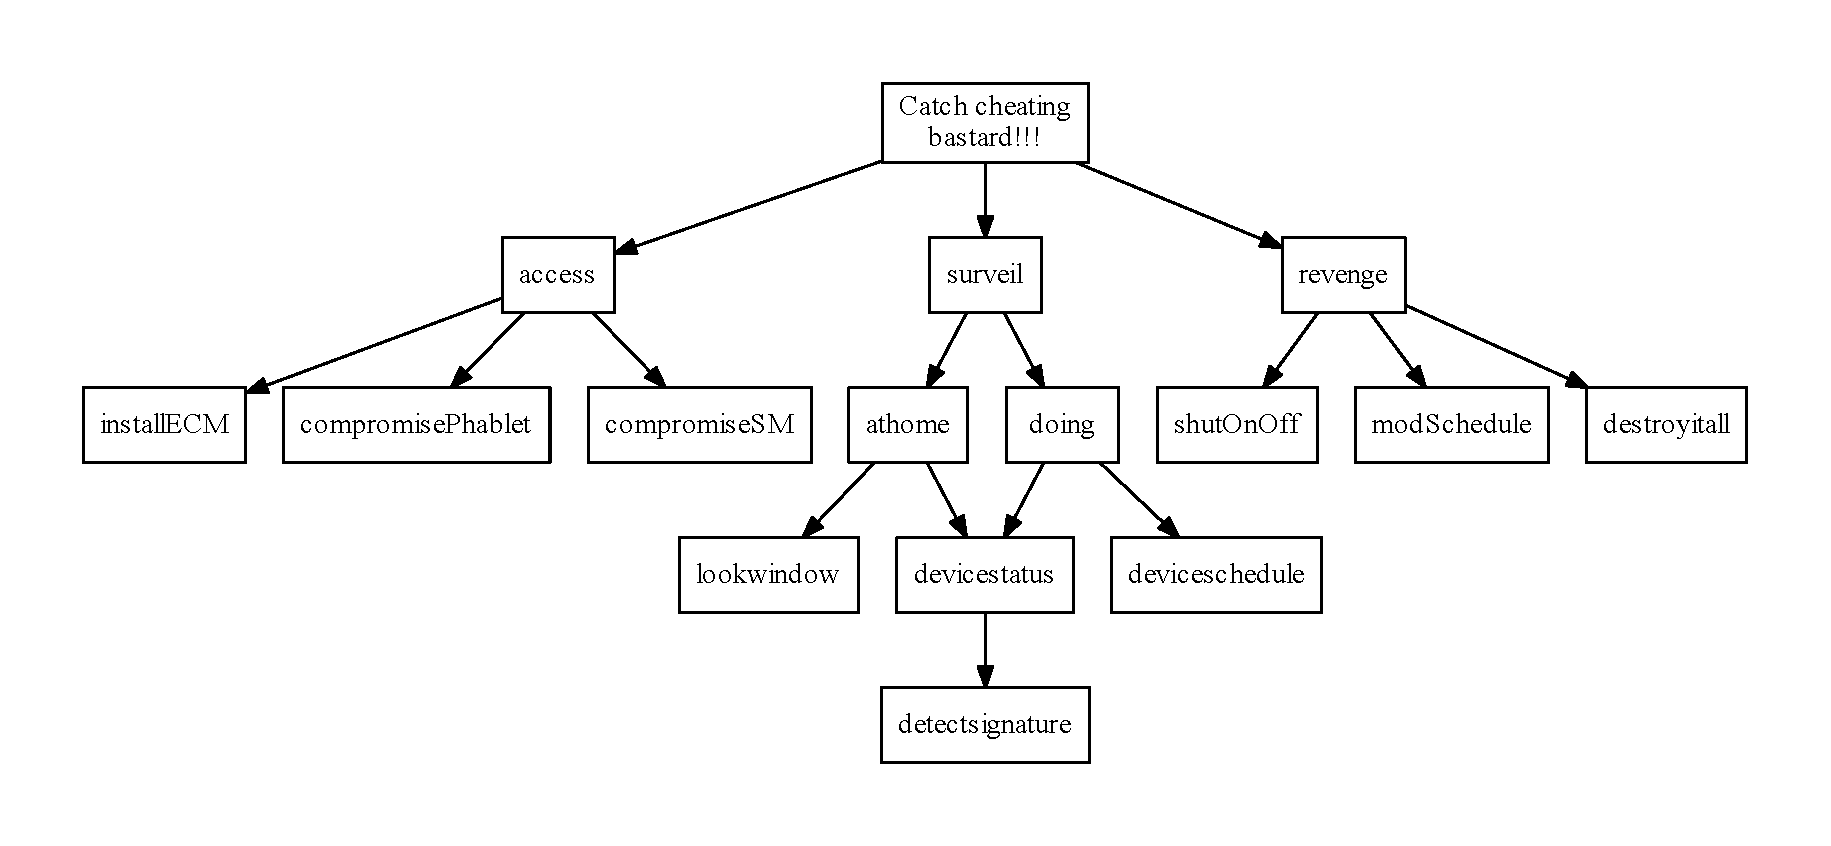
\includegraphics[angle=90,height=\textheight]{girlfriend_cheater_attack_tree}
	\caption{The Girlfriend vs Consumer -- "Catch cheating bastard" attack tree.}
	\label{fig:attack_trees:girlfriend:cheater}
	\mikael{Insert correct attack tree, someday...}
\end{figure}

The girlfriend is an actor with relation to the consumer, but unlike the other actors girlfriends usually can get away with more misdoings inside the consumer's property or house.

\subsubsection{"Catch cheating bastard"}

With this attack the girlfriend wishes to monitor the consumer, possibly with following revenge, if monitoring leads to the conclusion that the consumer was cheating on the girlfriend.
What distinguishes the girlfriend's attacks from the burglar or neighbour's is that she has increased access to the consumer's property, including the smart meter and related objects.

The attack tree can be seen in \cref{fig:attack_trees:girlfriend:cheater}.
There are three overall steps to the girlfriend's attack plan, these correspond to the direct descendants of the root node.

\paragraph{Access}
First of all she needs to gain access which can give her valuable insight into the doings of the consumer.
In relation to power consumption, she has three ways of accessing the consumer's data, which could give her the details she need to determine whether the consumer is home or not.

She could install an external consumption monitor\footnote{E.g. a TED (The Energy Detective) used in \cref {smart_meter_privacy}.} on the power grid in the house, giving her direct power consumption data.
Assuming that the consumer is using a tablet or other smart device to monitor his consumption, the girlfriend could gain access to one of these devices.
Finally, she could tamper directly with the smart meter, similar to the neighbour's or burglar's smart meter attacks.

\paragraph{Surveilance}
The main goal of this attack is to surveil and through this surveillance expose the consumer's misdeeds.
The nodes regarding devices are dependant on gained access through the \textit{access} sub-tree.

Her first option is physical presence, such as looking through a window.
However, assuming that she was able to somehow get hold of the consumer's power consumption data, she now has options to expose the consumer from a distance.

First of all, she could determine whether the consumer is home, and shouldn't be, or that he isn't home, but should be.
This can be done by looking at which devices are scheduled for tasks or from looking at the device power signatures.
The same method can be used to determine what the consumer is doing if he is home, such as brewing more coffee than usual or taking unusually long showers.

\paragraph{Revenge}
The final step of the attack plan is an optional cold dish of revenge.

She could of course destroy stuff by applying physical manipulation in one way or another.
However, if she wanted to get creative, she could use her previously gained access to the smart meter to manipulate the consumer psychologically.
She could turn on/shut off the consumer's appliances at inconvenient times.
If she really wanted to get cute, she could modify the appliances' schedules such as turning everything on at late night with low intervals.